\newpage
\section{Einstellungen für die PCB-Entwicklung in \enquote{Altium Designer}}\label{subsec:8.1}
%% Altium und Einstellungserklärung + Wichtige Layout-Faktoren
%Beim designen des Leiterplattenlayouts wurden die allgemeinen Altium-Einstellungen vorgenommen und auf die zu berücksichtigenden Layoutpunkte geachtet.
Beim \enquote{Layouten} der Schaltung in \enquote{Altium Designer} mussten einige wichtige Einstellungen vorab getätigt werden:\\
Wie da wären:
\begin{itemize}
	\item Arbeiten mit der Metrischen Einheit \enquote{mm}
	\item Layers benennen nach Vorgaben der Leiterplattenfertigung
	\item Kupferabstände
	\item Kupferbreite
	\item Lochdurchmesser und Restringeinstellungen für Vias
	\item Wärmefallen
	\item Restring für Pads
	\item Lochdurchmesser für Pads
\end{itemize}

\section{Designregeln für die PCB-Entwicklung}\label{subsec:8.2}
Beim Entwickeln einer Leiterplatte musste ständig auf wichtige Faktoren geachtet werden um eine Durchwegs EMV konforme, elektrisch wie auch mechanisch Stabile und Teils variable Schaltung zu erhalten.
Variabel daher weil es keine Prints für Serienreife sind, welche im Notfall auch mit anderen Bauteilen als den zuvor Vorgesehenen bestückt werden können.\\
Zu den Wichtigen Faktoren zählen:
\begin{itemize}
	\item EMV-Technische-Faktoren
	\begin{itemize}
		\item Kurze Leiterbahnen
		\item Durchdachtes Spannungsversorgungsnetz
		\item kleine Leiterschleifen
		\item Massefläche verwenden
		\item Anordnung der Bauteile
	\end{itemize}
	\item Ausnützen der Printfläche
	\item Mehrfach-Footprints ermöglichen für verschiedene Bauteile
	\item Mechanische Aufhängebohrungen vorsehen (in jeder Ecke des Prints)
	\item Beschriftung bei Möglichkeit vorsehen
\end{itemize}


\section{TDA2030}\label{sec:8.3}
Der TDA2030 ist ein für den Audio-Frequenzbereich optimierter OPV.
Dieser kann symmetrisch sowie auch asymmetrisch versorgt werden.
Eine typische Beschaltung ist im Datenblatt auch vorgegeben, welche auch verwendet wurde.
Der TDA2030 besitzt ein Pentawatt-Gehäuse, welches eine Kühlfläche besitzt.
Diese Kühlfläche hat das selbe Potential wie der mittlere Anschlusspin (Abb. \ref{fig:8.3.1}).\\
Es wird auch für geringfügigen Betrieb ein Kühlkörper empfohlen!
\begin{figure} [H]
	\centering
	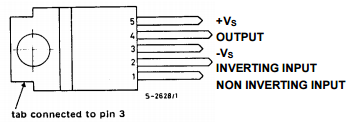
\includegraphics[width=1\textwidth]{img/Grundlagen/TDA2030/TDA2030Pinning.PNG}
	\caption[TDA2030-Pinning]{TDA2030-Pinning\footnotemark}
	\label {fig:8.3.1}
	%http://www.itisff.it/dip_eln/tda2030.pdf --> SnippingTool
\end{figure}
\footnotetext{http://www.itisff.it/dip\_eln/tda2030.pdf,\\Zugriff: 16.02.2017}
\begin{enumerate}
	\item Noninverting Input = Plus-Eingang des Verstärkers
	\item Inverting Input = Minus-Eingang des Verstärkers
	\item -Vs = negative Versorgungsspannung (bzw. Masse)
	\item Output = Verstärkerausgang
	\item +Vs = positive Versorgungsspannung		
\end{enumerate}

\newpage
\subsection{Absolute Maximalwerte}\label{subsec:8.3.1}
Diese Werte wurden zu aller erst mit den Bedingungen an der Schaltung verglichen, da sie ein sehr genaue, kurze Übersicht über den Baustein liefern. (Abb. \ref{fig:8.3.1.1})
\begin{figure} [H]
	\centering
	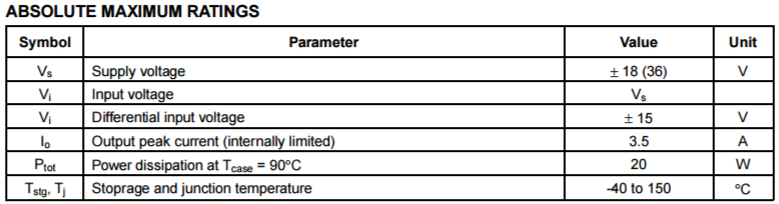
\includegraphics[width=1\textwidth]{img/Grundlagen/TDA2030/TDA2030MaximumRatings.PNG}
	\caption[TDA2030-Maximum Ratings]{TDA2030-Maximum Ratings\footnotemark}
	\label {fig:8.3.1.1}
	%http://www.itisff.it/dip_eln/tda2030.pdf --> SnippingTool
\end{figure}
\footnotetext{http://www.itisff.it/dip\_eln/tda2030.pdf,\\Zugriff: 16.02.2017}

\subsection{TDA2030-Grundschaltung}\label{subsec:8.3.2}
Ein wichtiges Bauelement in der Grundschaltung(Abb. \ref{fig:8.3.2.1}) sind die Dioden. Sie schützen den angeschlossenen Lautsprecher vor Überspannungsspitzen.\\
Das Spannungsteiler am Plus-Eingang (Pin1) des OPVs ist da um den Arbeitspunkt des TDA2030 festzulegen.
In diesem Fall bei asymmetrischer Versorgung soll dieser $\frac{Vcc}{2}$ betragen.\\
Das Widerstandsverhältnis am Minus-Eingang (Pin2) des OPVs von 150k Ohm zu 4,7k Ohm liefert die Verstärkung der Schaltung.
Hier wäre es dementsprechend eine Verstärkung von ungefähr x32 .\\
Viele vereinzelte Kondensatoren sind zum Entstören und gegen mögliches Schwingen der Schaltung vorgesehen.\\
Der Große-Ausgangs-ELKO wird deshalb verbaut um keine verschleppte Gleichspannung am Lautsprecher unnötigerweise anzulegen.
Gleichspannung ist an einem Lautsprecher weder hörbar (Frequenz = 0Hz) noch sinnvoll und kann den Lautsprecher beschädigen.
Der Kondensator lädt sich einmal mit dieser Gleichspannung auf und lässt die Wechselspannung ohne weiteres passieren.\\\\
Ein weiteres wesentliches Bauelement ist das \enquote{Boucherot-Glied}, ein in Serie geschalteter Kondensator und Widerstand von der Ausgangsleitung des Verstärkers gegen Masse, noch vor dem Ausgangs-ELKO.
Es dient zur Widerstandsanpassung im höheren Audio-Frequenzbereich, da der Lautsprecher einen induktiven Impedanzabfall aufweist, wird dieser mit dem kapazitiven Impedanzanstieg in diesem Bereich kompensiert.
So bleibt die Impedanz im Arbeitsbereich des Verstärkers im wesentlichen die selbe.
Ein weiterer Vorteil ist, dass Frequenzen über der Grenzfrequenz des \enquote{Boucherot-Glieds} wie ein Kurzschluss behandelt werden und so mögliche auftretende Schaltfrequenzen gedämpft werden und nicht andere folgende Schaltungen beeinflussen können.\\\\
Die Schaltung ist grundsätzlich für symmetrische und asymmetrische Versorgungsspannung ausgelegt. 
Die Schaltung ist für 4 und 8 Ohm Lautsprecher spezifiziert.
\begin{figure} [H]
	\centering
	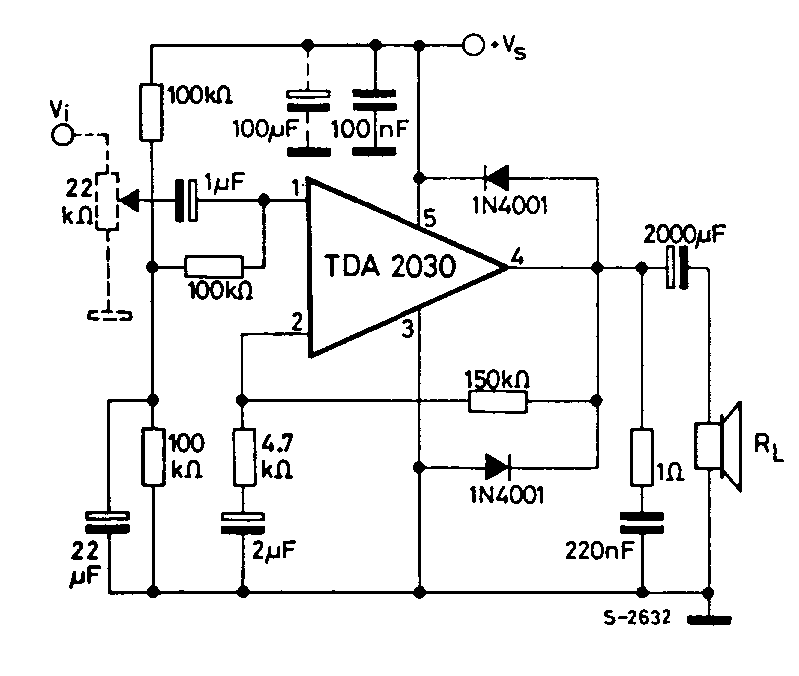
\includegraphics[width=1\textwidth]{img/Grundlagen/TDA2030/TDA2030-Grundschaltung.png}
	\caption[TDA2030-Grundschaltung]{TDA2030-Grundschaltung\footnotemark}
	\text (Die im Bild vorhandenen Werte müssen nicht der entwickelten Schaltung entsprechen. Es dient nur zu Veranschaulichung der Schaltung.)
	\label {fig:8.3.2.1}
	%http://www.mikrocontroller.net/attachment/79272/Schaltung.png
\end{figure}
\footnotetext{http://www.mikrocontroller.net/attachment/79272/Schaltung.png,\\Zugriff: 16.02.2017}

\subsection{Leistungstransistor-Schaltung}\label{subsec:8.3.3}
Durch das Erweitern der TDA2030-Grundschaltung(Kap. \ref{subsec:8.3.2}) mit zwei Leistungstransistoren wird die Schaltung leistungsfähiger.
Die Transistoren schalten Ströme über den maximalen schaltbaren Strömen des TDA2030. Während des Normalbetriebes fließt kein Strom durch die Transistoren, sobald aber eine Grenze erreicht wird, wird grundsätzlich mit den Transistoren gearbeitet.
Um die Schaltschwelle der Leistungstransistoren festzulegen wird ein kleiner Widerstand von der Versorgungsspannung gegen den Basis-Anschluss des Transistors geschallten.
Beziehungsweise wird dieser Widerstand von der Negativen Versorgungsspannung, oder in diesem Fall von Masse, gegen den Basis-Anschluss des Leistungstransistors geschaltet.
Des weiteren sind die Leistungstransistoren im besten Fall aus der selben Familie.
Verwendet wird ein PNP-Leistungstransistor für die positive Halbwelle des Signals und ein NPN-Leistungstransistor für die negative Halbwelle.
\begin{figure} [H]
	\centering
	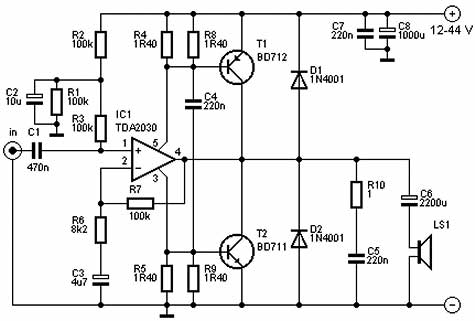
\includegraphics[width=1\textwidth]{img/Grundlagen/TDA2030/TDA2030-Leistungstransschaltung.jpg}
	\caption[TDA2030-Leistungstransistorschaltung]{TDA2030-Leistungstransistorschaltung\footnotemark}
	\text (Die im Bild vorhandenen Werte müssen nicht der entwickelten Schaltung entsprechen. Es dient nur zu Veranschaulichung der Schaltung.)
	\label {fig:8.3.3.1}
	%http://www.audiofanatic.it/Schemi/Tipo/Stato_solido/chip/pic_chip/TDA_2030_BD711_712.jpg
\end{figure}
\footnotetext{http://www.audiofanatic.it/Schemi/Tipo/Stato\_solido/chip/pic\_chip/TDA\_2030\_BD711\_712.jpg,\\Zugriff: 16.02.2017}

\subsection{H-Brückenschaltung der TDA2030-Verstärkerschaltung}\label{subsec:8.3.4}
Um noch mehr aus dem TDA2030 herauszuholen kann man zwei dieser Verstärker in H-Brücke (Abb. \ref{fig:8.3.4.1}) gegeneinander schalten.
Ein TDA2030 verstärkt das originale Signal, währenddessen der Zweite das um 90° phasenverschobene Signal erhält und dieses verstärkt.
Das hat zur Folge das während der eine TDA2030 die positive Halbwelle verstärkt der zweite die negative Halbwelle verstärkt.
Dies bewirkt einen größeren Hub, da der eine Verstärker bei maximaler Auslenkung die positive Versorgungsspannung erreicht, während der zweite die negative Versorgungsspannung erreicht.
So erhält man mit zwei TDA2030 den doppelten Ausgangspegel des Signals.\\
Einziger Nachteil dieser Konstellation: Zwischen den beiden Verstärkern gibt es keinen Massebezug.
Beim Messen der Schaltung ist Vorsicht geboten, da beim Anschließen der Tastkopf-Masse, je nach anliegendem Signal, der eine oder der andere Verstärker beschädigt werden kann(Kurzschluss!).\\
Es kann in diesem Fall auch die Leistungstransistorschaltung in H-Brücke geschaltet werden um noch mehr aus der Sache heraus zu holen.
\begin{figure} [H]
	\centering
	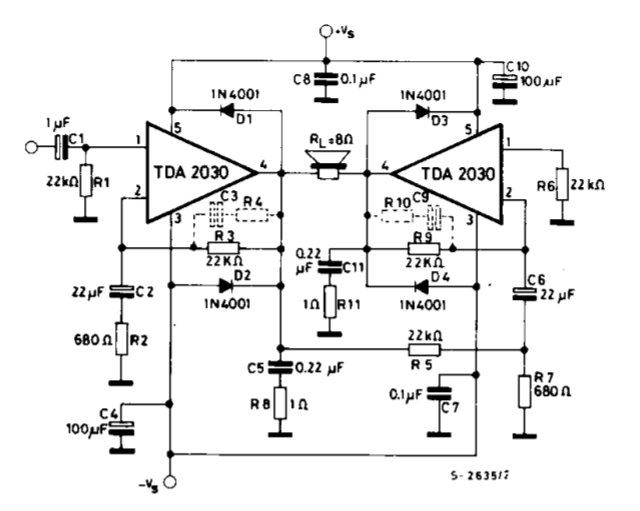
\includegraphics[width=1\textwidth]{img/Grundlagen/TDA2030/TDA2030-H-Bruecke.PNG}
	\caption[TDA2030-H-Brückenschaltung]{TDA2030-H-Brückenschaltung\footnotemark}
	\text (Die im Bild vorhandenen Werte müssen nicht der entwickelten Schaltung entsprechen. Es dient nur zu Veranschaulichung der Schaltung.)
	\label {fig:8.3.4.1}
	%http://www.itisff.it/dip_eln/tda2030.pdf --> SnippingTool
\end{figure}
\footnotetext{http://www.itisff.it/dip\_eln/tda2030.pdf,\\Zugriff: 16.02.2017}

\begin{comment}
\subsection{Asymmetrische Spannungsversorgung}\label{subsec3.2.5}
Bedingt durch eine asymmetrische Spannungsversorgung (zB. 0 und 12V), muss am OPV ein Arbeitspunkt eingestellt werden.
Dabei handelt es sich um ein absichtliches Anheben des Signals in Y-Richtung bei einem Spannungs-Zeit-Verlauf, sodass die negative Halbwelle des Signals nicht verloren geht.
Die negative Halbwelle würde sonst in den negativen Spannungsbereich reichen wollen, aber dieser ist mit negativer Versorgungsspannung von 0V, also Masse, nicht vorhanden.\\
Dieser Effekt tritt auf, da ein Audio-Signal in der Regel ein symmetrisches Signal ist und eine asymmetrische Versorgungsspannung des Verstärkers dementsprechend die Symmetrie stört.\\
Um die Symmetrie jedoch trotz asymmetrische Spannungsversorgung beizubehalten, wird ein Arbeitspunkt eingestellt.
Dafür wird an dem Plus-Eingang des OPVs über eine Spannungsteiler-Schaltung aus zwei Widerständen das benötigte $\frac{Vcc}{2}$ angelegt.
\end{comment}


\section{Filter}\label{sec:8.4}
Es wurde nach einem möglichst steilen, im Durchlassbereich linearen und einfachen Filter gesucht.
Man hat sich für ein \enquote{Aktives-Filter 2.Ordnung} entschieden, dabei wurde die \enquote{Butterworth-Schaltung} bevorzugt.
Wegen seiner geringen Welligkeit im Durchlassbreich und einer Dämpfung von $\frac{-20dB}{Dek.}$ .
Dies bedeutet, dass bei einer Tiepfass-Filterung eine Frequenz die 10mal größer ist als die Grenzfrequenz einen um $\frac{1}{10}$ kleineren Pegel aufweist, als die Grenzfrequenz.\\
\begin{comment}
Zur Regelung wird an den Eingängen (Rechts, Links) und bei der Schaltung (Abb. \ref{fig:8.2.5.1}) auch am Ausgang, jeweils ein Potentiometer in der Größenordnung von 1kOhm verbaut.
Diese dienen zur Anpassung der Amplitude des ein- und ausgehenden Signals, um mögliche Übersteuerungen zu vermeiden.
\end{comment}

\subsection{Butterworth-Filter 2. Ordnung}\label{subsec:8.4.1}
Die Grundschaltung eines \enquote{Butterworth-Filters 2. Ordnung} ist für verschiedene Grenzfrequenzen dieselbe, lediglich die Bauteilwerte variieren.
Auch die Schaltung der verschiedenen Grundfilterarten ist unterschiedlich. \\
Die da wären: 
\begin{itemize}
	\item Hochpass-Filter
	\item Tiefpass-Filter
	\item Bandpass-Filter
\end{itemize}
Ein Butterworth-Tiefpass-Filter 2. Ordnung besteht hauptsächlich aus einem OPV, drei Widerständen und zwei Kondensatoren.
Deren Anordnung ist ausschlaggebend für das Tiefpass-Filter (Abb. \ref{fig:8.4.1.1}).
Dieses Filter lässt alle Frequenzen unterhalb seiner Grenzfrequenz durch.\\ 
Bedingt durch das Beschalten des OPVs wird das Ausgangssignal invertiert, was hier keine gröberen Folgen mit sich bringt.\\ 
Am Plus-Eingang des OPVs wird entweder Masse bei symmetrischer Spannungsversorgung, oder $\frac{Vcc}{2}$ bei asymmetrischer Spannungsversorgung angelegt.
\begin{figure} [H]
	\centering
	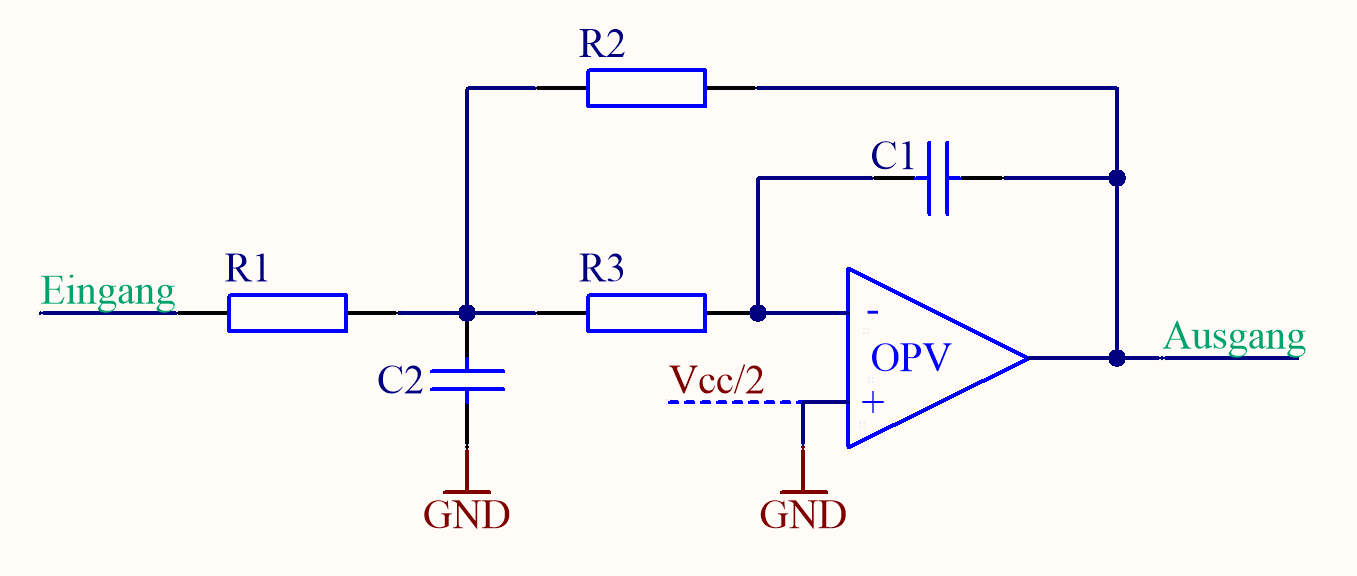
\includegraphics[width=1\textwidth]{img/Print3/TPFilterButterworth2Ordnung.PNG}
	\caption{Butterworth-Tiefpass-Filter 2. Ordnung}
	\label {fig:8.4.1.1}
	%Selbst generiert in Altium
\end{figure}
Das Bandpass-Filter(\ref{fig:8.4.1.2}) besteht aus drei Widerständen, zwei Kondensatoren und einem OPV, jedoch mit anderer Anordnung als bei dem Tiefpass-Filter.
Dieses Filter lässt alle Frequenzen oberhalb seiner Unteren-Grenzfrequenz und unterhalb seiner Oberen-Grenzfrequenz durch.
\begin{figure} [H]
	\centering
	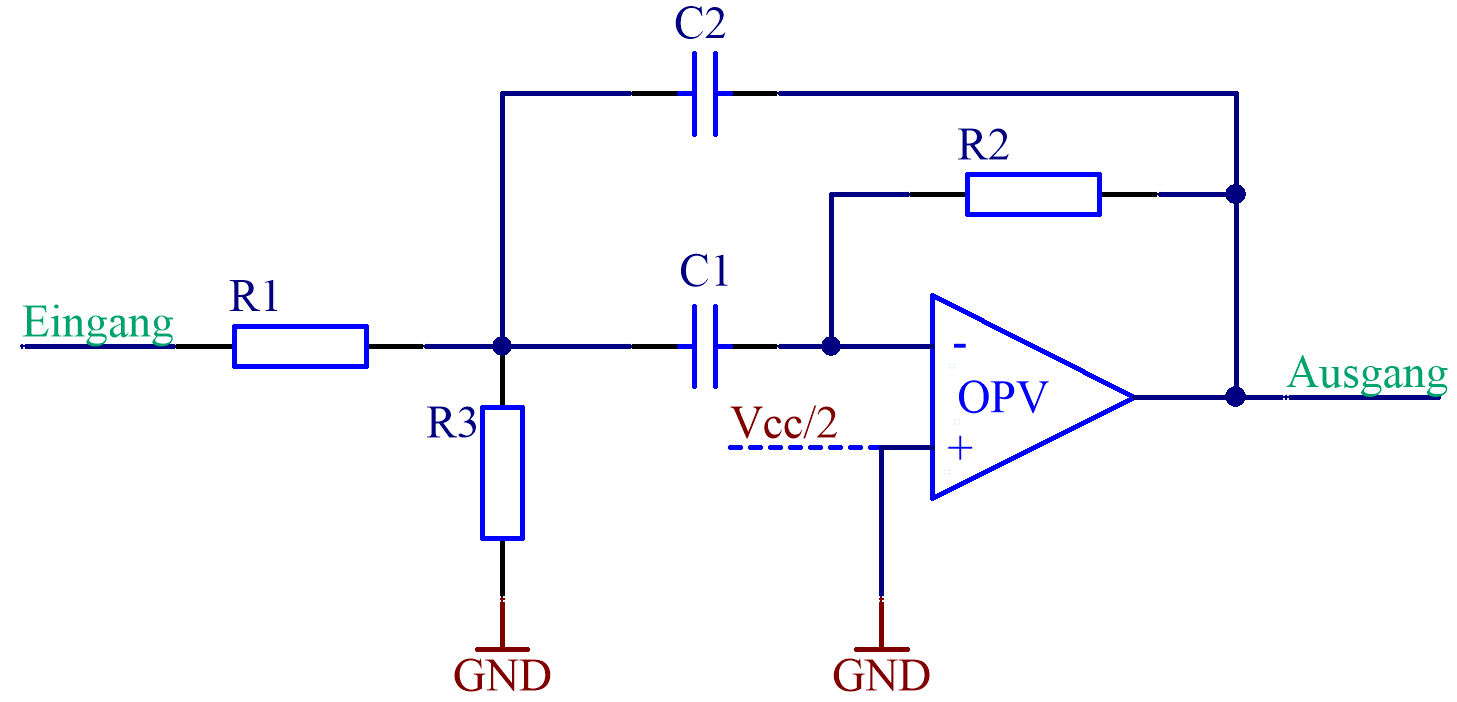
\includegraphics[width=1\textwidth]{img/Print4/BPFilter-Butterworth2Ordnung.PNG}
	\caption{Butterworth-Bandpass-Filter 2. Ordnung}
	\label {fig:8.4.1.2}
	%Selbst generiert in Altium	
\end{figure}
Das Hochpass-Filter(\ref{fig:8.4.1.3}) hat wieder eine ähnliche Konstruktion.
Dieses besteht aus drei Kondensatoren, zwei Widerständen und einem OPV.
Wiederum in mit bestimmter Anordnung.
Dieses Filter lässt alle Frequenzen oberhalb seiner Grenzfrequenz durch.
\begin{figure} [H]
	\centering	
	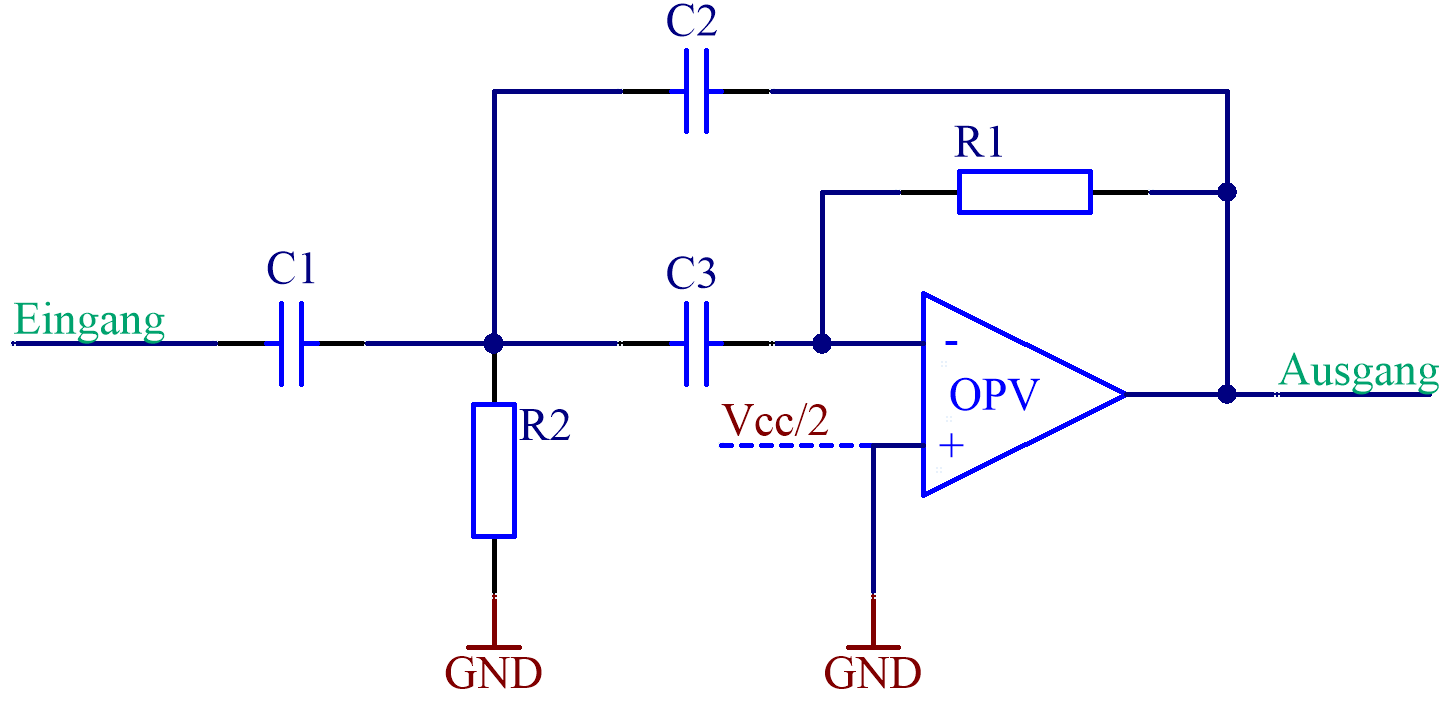
\includegraphics[width=1\textwidth]{img/Print4/HPFilter-Butterworth2Ordnung.PNG}
	\caption{Butterworth-Hochpass-Filter 2. Ordnung}
	\label {fig:8.4.1.3}
	%Selbst generiert in Altium	
\end{figure}

% WIRD SCHON BEI GRUNDLAGEN ERKLÄRT!
%\section{Satelliten-Lautsprecher}\label{sec:8.5}
%Satellitenlautsprecher sind meist passive Lautsprecher, die durch ein Aktives-Element betrieben werden.
%Da es sich bei dem Satellitensystem meist um ein Paar oder mehr Boxen handelt und diese räumlich weiter entfernt voneinander stehen, können Stereo-Effekte verwendet und mit dem reinen Stereo-Eingangssignal gearbeitet werden.
%Eine Aufteilung des Signals in Linke- und Rechte-Satellitenbox/en muss jedoch schon getroffen werden, um die Effekte richtig zu erhalten.

\section{Nicht invertierende Verstärker - OPV-Grundschaltung}\label{sec:8.5}
Die hauptsächlichen Eigenschaften eines solchen Verstärkers liegen in der Phasengleichheit am Ein- und Ausgang der Schaltung und am wichtigsten, in der Verstärkung. \\
Um eine Verstärkung zu erhalten wird am invertierten Eingang (\ref{fig:8.5.1}), oder umgänglicher am Minus-Eingang des OPV ein Rückkopplungsnetz aus zwei Widerständen gebaut.
Diese bewirken, dass eine Verstärkung \enquote{Vu} möglich ist.
Diese wird wie folgt berechnet: Vu = $\frac{R2+R1}{R1}$ .
Aus der Formel geht hervor das R2 im Verhältnis zu R1 normalerweise größer sein sollte um eine nennenswerte Verstärkung zu erhalten.
Die Verstärkung funktioniert aus einem einfachen Grund.
Wenn am Eingang ein Signal anliegt möchte der OPV nach seiner Natur den selben Wert wie am + Eingang auch am - Eingang haben, er regelt nach.
Das heißt der Spannungsunterschied Upn soll gegen 0 gehen.
Wird nun künstlich das Nachregeln beeinflusst, indem man einen Spannungsteiler einbaut, regelt der OPV den Ausgang höher als er eigentlich müsste, er Verstärkt also.
Der Verstärker ist jedoch durch seine Versorgungsspannung begrenzt, soll heißen wenn man ein Verstärkung von 10 erwartet bei einem Eingangssignal von 1 Volt und einer Versorgungsspannung von 5 Volt, dann ist das Signal nie 10 Volt groß.
Ein OPV-Verstärker kann auch übersteuert werden.
Das passiert wenn man ihn, wie bereits vorher erläutert, zu viel Eingangssignal liefert in Abhängigkeit zu der Verstärkung und der Versorgungsspannung.
So kommt es das wenn der OPV übersteuert ein Sinus kein Sinus mehr ist sonder vielleicht gar zum Rechteck wird, da die Ober- und Untergrenze die positive und negative Versorgungsspannung bietet.
\begin{figure} [H]
	\centering	
	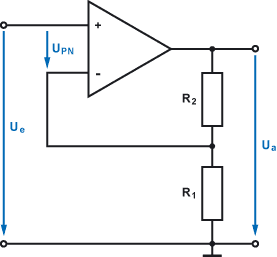
\includegraphics[width=0.6\textwidth]{img/Grundlagen/OPV-Verstaerker/OPV-VerstaerkerGrundschaltung.png}
	\caption[Nicht invertierender Verstärker - OPV-Grundschaltung]{Nicht invertierender Verstärker - OPV-Grundschaltung\footnotemark}
	\label {fig:8.5.1}
	%http://www.elektronik-kompendium.de/sites/slt/schalt/02101511.gif
\end{figure}
\footnotetext{http://www.elektronik-kompendium.de/sites/slt/schalt/02101511.gif,\\Zugriff: 16.02.2017}

\subsection{Asymmetrische Versorgung eines OPV's}\label{subsec:8.5.1}
Beim Arbeiten mit OPV-Verstärkerschaltungen muss die Symmetrie der Verstärkung beachtet werden.
Bei einer asymmetrischen Versorgung muss daher beachtet werden, dass ein bestimmter Arbeitspunkt eingestellt wird.
Dieser ist dafür da um die Asymmetrie durch die Spannungsversorgung wieder auszugleichen.
Dafür wird am Eingang ein Spannungsteiler dimensioniert welcher in Mitte von diesem $\frac{Vcc}{2}$ erzeugt.
Dies erfolgt über zwei gleichgroße Widerstände, die zumeist im Bereich vom Kilo-Ohm liegen.
Sie werden in Serie von Vcc gegen Masse gelegt, somit kann zwischen den beiden Widerständen $\frac{Vcc}{2}$ abgegriffen werden.
Somit liegt das Eingangssignalgrundpegel in mitten der Versorgungsspannung.
D.h. der Spannungsunterschied zur positiven Versorgungsspannung ist der selbe wie zur negativen Versorgungsspannung (Masse). 

% IN DIE GRUNDLAGEN VERSCHOBEN!
%\newpage
%\section{Versorgungskonzept} \label{sec:8.6}
%Die gesamte Box soll portabel sein, d.h. ohne externe Stromzufuhr funktionieren.
%Dafür ist ein Akku notwendig.
%Nach einigen Überlegungen haben wir uns für einen Blei-Vlies-Akku entschieden.
%Gründe dafür sind:
%\begin{itemize}
%	\item Geringe Kosten
%	\item Einfache Beschaltung
%	\item Geringere Gefahr gegenüber Lithium-Akkus
%	\item Wegen Vlies-Technik: Kein Auslaufen von chemischen Substanzen
%\end{itemize}
%Dieser Akku versorgt grundsätzlich die Elektronik mit 12 V.
%Da aber mit dieser, relativ geringen, Spannung nur eher kleine Leistungen zu erwarten sind, kam die Idee auf, die Verstärker bei externer Versorgung durch das Stromnetz mit einer größeren Spannung (24 V) zu versorgen.
%Um das zu realisieren wird ein Netzteil, in unserem Fall ein Schaltnetzteil benötigt.
%Falls das Gerät am externen Stromnetz hängt, wird die Versorgung der Verstärker automatisch mithilfe eines passenden Relais umgeschaltet.
%Diese Lösung wurde gewählt, da sie sehr simpel ist und gut funktioniert.
%Veranschaulicht wird das Konzept durch diese Schaltung:
%\begin{figure} [H]
%	\centering	
%	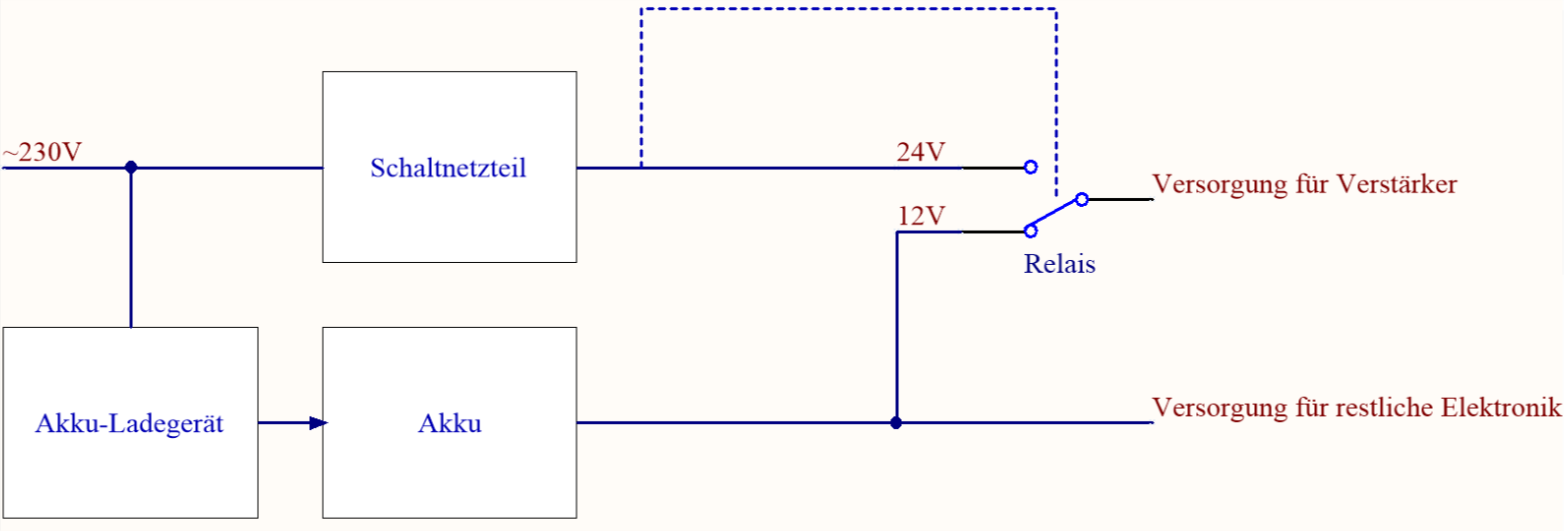
\includegraphics[width=1\textwidth]{img/Grundlagen/Versorgung.png}
%	\caption{Versorgungskonzept}
%	\label {fig:8.6.1}
%\end{figure}

\section{Welligkeit} \label{sec:8.6}
Die Welligkeit gibt den Toleranzbereich um einen idealen(linearen) Frequenzgang an.
Das bedeutet wenn ein Weißes-Rauschen mit einem definierten Pegel an der Membran abgestrahlt wird, darf der Pegel über den Frequenzverlauf im Welligkeitsbreich variieren, ohne das es als kritisch empfunden werden muss. \\
Für Lautsprechermessungen ist eine Welligkeit im \enquote{Consumer-Bereich} von 10dB und im \enquote{HiFi-Bereich} von 6dB üblich.
So darf ein Consumer-Lautsprecher bei einem definierten Pegel von 80dB über den ganzen Messbereich maximal +/- 5dB variieren, d.h. im Bereich zwischen 75 dB und 85 dB.
Fällt der Pegel viel mehr als der definierte Welligkeitsbereich, wird der Lautsprecher zumeist gefiltert.
Dadurch ist es möglich einen anderen Lautsprecher diese Bereich zu übernehmen und die Schwäche des anderen auszubessern.\\ \\
Ziel eines Lautsprechersystems ist es über den ganzen Audiobereich, 20 Hz bis 20 kHz, einen linearen bzw. näherungsweise linearen Frequenzgang zu erhalten.




